% ─── Appendix / Backup slides ─────────────────────────────────────────────────

% ─── Backup: copy of Final Results slide (big table) ──────────────────────────
\begin{frame}{Backup: Final Results — INT4+LoRA Beats INT8+ADC PTQ on Llama-3.2-1B}

  \vspace{0.3em}
  \begin{center}
  \renewcommand{\arraystretch}{1.25}
  \setlength{\tabcolsep}{3.0pt}
  \scriptsize
  \resizebox{\textwidth}{!}{%
  \begin{tabular}{@{}l r r r r r r r r r r r@{}}
    \toprule
      & \multicolumn{2}{c}{\textbf{PPL} ($\downarrow$)}
      & \multicolumn{8}{c}{\textbf{Accuracy} \% ($\uparrow$)}
      & \\
    \cmidrule(lr){2-3} \cmidrule(lr){4-11}
    \textbf{Method} &
      \textbf{Wiki} & \textbf{C4} &
      \textbf{HSwag} & \textbf{MMLU} & \textbf{WinGr} &
      \textbf{ARC-E} & \textbf{ARC-C} & \textbf{PIQA} &
      \textbf{OBQA} & \textbf{BoolQ} & \textbf{Avg} \\
    \midrule
    bfloat16          & \textbf{8.68}  & \textbf{13.13} & \textbf{64.19} & \textbf{32.15} & 63.06 & 61.83 & 36.77 & 74.70 & 37.40 & 63.91 & \textbf{54.25} \\
    \midrule
    INT8 PTQ          &  8.69 & 13.15 & 64.17 & 31.89 & \textbf{63.38} & \textbf{69.82} & \textbf{39.16} & \textbf{75.79} & \textbf{39.20} & \textbf{64.22} & \textbf{55.95} \\
    INT8 + ADC PTQ    & 16.85 & 29.56 & 45.04 & 26.83 & 56.59 & 48.44 & 28.84 & 64.36 & 30.00 & 59.63 & 44.97 \\
    \midrule
    INT4 PTQ          & 14.13 & 22.83 & 51.98 & 24.86 & 55.25 & 60.44 & 33.02 & 69.48 & 32.00 & 62.11 & 48.64 \\
    INT4 + ADC PTQ    & 26.66 & 45.62 & 40.03 & 24.41 & 53.43 & 42.63 & 26.02 & 61.70 & 27.00 & 60.67 & 41.99 \\
    INT4 + ADC + LoRA & \textbf{14.03} & \textbf{23.20} & \textbf{49.96} & \textbf{25.72} & \textbf{53.67} & \textbf{54.63} & \textbf{29.27} & \textbf{68.06} & \textbf{34.60} & 60.67 & \textbf{47.07} \\
    \bottomrule
  \end{tabular}}
  \end{center}

  \vspace{0.4em}
  \begin{center}\scriptsize
  PPL lower is better; accuracy higher is better.  \textbf{Avg} = unweighted
  mean of the 8 lm-evaluation-harness accuracies.  Rows without ``+ ADC'' are
  integer-only baselines (no ADC step); rows with ``+ ADC'' include the
  finite-resolution ADC ($b_a{=}8$, fixed $\delta$).
  \end{center}
\end{frame}

\begin{frame}{Backup: $\alpha$-Sweep — $\alpha{=}0.5$ Wins}
  \begin{center}
    
\includegraphics[width=0.8\linewidth]{figs/plot_alpha_sweep.pdf}
  \end{center}
\end{frame}

\begin{frame}[shrink=10]{Backup: Rotation Line of Work}
  \footnotesize
  \textbf{The rotation line of work.}\\[0.3em]
  Insert an orthogonal $T$ so that $W T^{-1}\cdot T x = Wx$ and $Tx$ is easier to quantise:
  \begin{center}
  \begin{tikzpicture}[every node/.style={font=\small},
                     node distance=0.4cm,
                     box/.style={draw, rounded corners=2pt,
                                 minimum width=2.0cm, minimum height=0.55cm,
                                 align=center}]
    \node[box, fill=mygray!15] (q) {QuaRot\\\small Hadamard, fixed};
    \node[box, fill=mygray!30, right=of q] (s) {SpinQuant\\\small trained rotations};
    \node[box, fill=myorange!30, right=of s] (f) {\textbf{FlatQuant}\\\small Kron.\ + per-layer};
    \draw[-{Latex}, thick] (q) -- (s);
    \draw[-{Latex}, thick] (s) -- (f);
  \end{tikzpicture}
  \end{center}

  \vspace{0.5em}
  \textbf{Why FlatQuant for our work:}
  \begin{itemize}
    \setlength\itemsep{0.3em}
    \item \emph{trainable} — we can add objectives (ADC-aware);
    \item \emph{Kronecker} ($T = T_1 \otimes T_2$) — memory \& compute $\mathcal{O}(\sqrt{d})$;
    \item per-projection rotations fold naturally into block-wise calibration.
  \end{itemize}
\end{frame}

% ──────────────────────────────────────────────────────────────────────────────

\begin{frame}[shrink=28]{Why ADC is Hard for LLMs: the Outlier Dilemma}
  \textbf{LLM activations are heavy-tailed.}
  A tiny fraction of channels carry magnitudes $10\text{--}100\times$ larger
  than the rest \textit{\small (Dettmers 2022; Xiao 2023)}.

  \vspace{0.3em}
  \begin{columns}[T]
    \begin{column}{0.42\textwidth}
      \begin{center}
        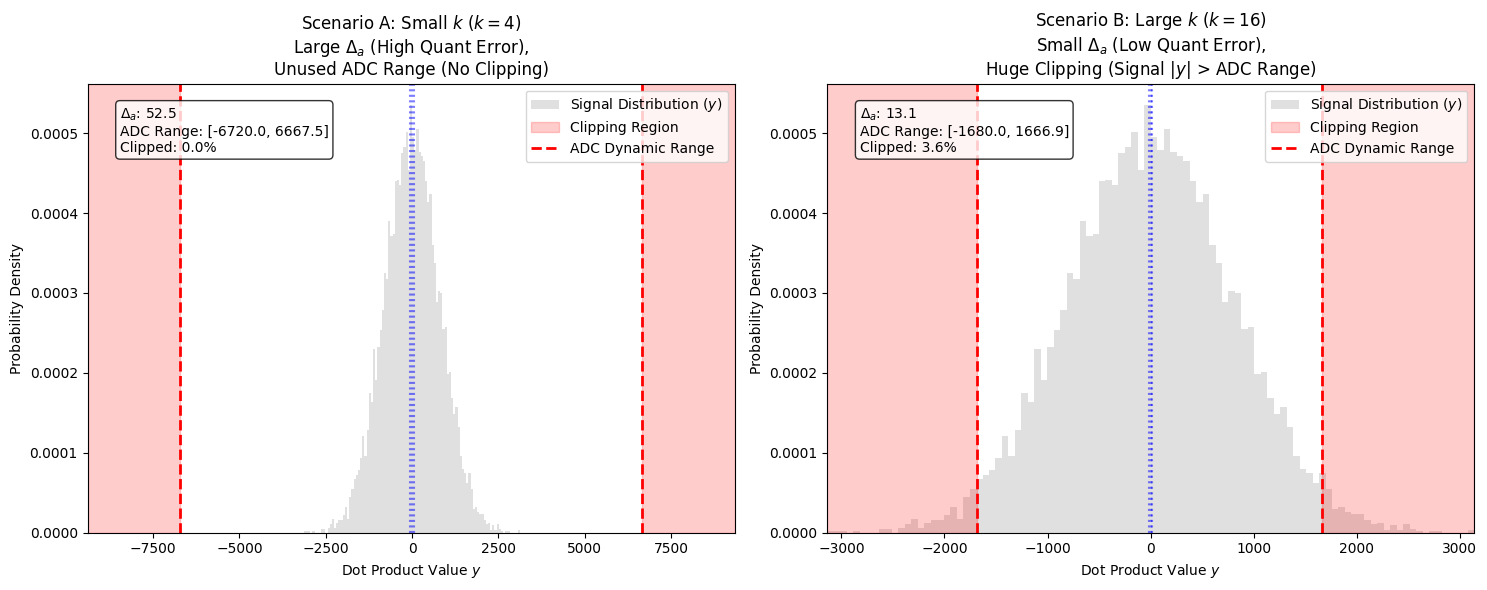
\includegraphics[width=\linewidth]{figs/dead_zone.png}
      \end{center}
      \vspace{-0.2em}
      \begin{center}\tiny Llama-3.2-1B \texttt{q\_proj} dot-product distribution, two ADC step sizes\end{center}
    \end{column}

    \begin{column}{0.57\textwidth}
      \footnotesize
      \textbf{Why we can't just pick a good $k$:}\\[0.2em]
      \begin{tabular}{@{}p{0.44\linewidth} p{0.48\linewidth}@{}}
        \toprule
        \textbf{\color{myred}Large $k$ (fine $\delta$)} &
        \textbf{\color{mybluedark}Small $k$ (coarse $\delta$)} \\
        \midrule
        outliers saturate the ADC range \newline
          $\Rightarrow$ heavy \emph{clipping} & outliers stay in range \\
        model loses critical channels & dynamic range wasted on outliers \\
        good ADC SNR on bulk & bulk collapses into \emph{dead zone} \\
        \alert{bad downstream accuracy} & \alert{bad ADC SNR everywhere} \\
        \bottomrule
      \end{tabular}
    \end{column}
  \end{columns}

  \vspace{0.5em}
  \begin{block}{Takeaway}
    \small
    Hardware-fixed $\delta$ $+$ heavy-tailed activations
    $\Rightarrow$ \textbf{no single $k$ works}.
    The algorithm must reshape $x$ and $w$ \emph{before} they hit the array
    so that $y$ lands in the ADC's usable range.
  \end{block}
\end{frame}

% ──────────────────────────────────────────────────────────────────────────────

\begin{frame}[shrink=20]{Backup: Complete INT8 Results (v2)}
  \footnotesize
  \textbf{Setup:} Llama-3.2-1B, w8a8, 128 calibration samples. Testing two ideas on top of baseline FlatQuant: (1) \emph{bin-centre loss} — pushes $y_{\rm int}$ toward ADC bin centres during PTQ; (2) \emph{propagated calibration} — each block sees ADC-quantised inputs from the previous block, matching inference conditions. Key finding: propagation gives a $2\times$ ADC PPL drop; bin-centre loss alone gives nothing.
  \vspace{0.3em}
  \begin{center}
  \small
  \begin{tabular}{llcccc}
    \toprule
    Experiment & Description & $\bypass$ & $\adcppl$ & dead\_rate \\
    \midrule
    baseline       & FlatQuant w8a8               & 10.01 & 28.86 & 10.3\% \\
    center mid     & bin-centre $\lambda=0.1$      & 10.01 & 28.86 & 10.3\% \\
    prop           & propagated calibration        & 11.01 & \better{14.55} & 10.3\% \\
    prop+center    & propagated + bin-centre       & 11.00 & \best{14.41} & 10.3\% \\
    \bottomrule
  \end{tabular}
  \end{center}
\end{frame}

% ──────────────────────────────────────────────────────────────────────────────

\begin{frame}[shrink=20]{Backup: Complete INT4 v2 Alpha-Sweep}
  \footnotesize
  \textbf{Setup:} Llama-3.2-1B, w4a4, 1024 samples. Sweeping $\alpha$ in the mixed loss $\mathcal{L}(\alpha)=(1{-}\alpha)\mathcal{L}_{\rm FP}+\alpha\mathcal{L}_{\rm ADC}$. $\alpha{=}0$ = clean FP inputs only; $\alpha{=}1$ = ADC-noisy inputs only. Gap = ADC PPL / no-ADC PPL. Last two rows add diagonals and staged training on top of $\alpha{=}0.5$.
  \vspace{0.3em}
  \begin{center}
  \small
  \begin{tabular}{llccc}
    \toprule
    Experiment & $\alpha$ & $\bypass$ & $\adcppl$ & gap \\
    \midrule
    baseline\_1024        & 0.0 & 19.80 & 56.83 & $\times$2.87 \\
    prop\_full\_1024      & 1.0 & 30.32 & 40.20 & $\times$1.32 \\
    propalpha\_075\_1024  & 0.75 & 27.46 & 35.92 & $\times$1.31 \\
    propalpha\_05\_1024   & 0.5 & 24.24 & \better{31.22} & \best{$\times$1.29} \\
    propalpha\_025\_1024  & 0.25 & 21.65 & 32.35 & $\times$1.49 \\
    add\_diag + $\alpha$=0.5 & 0.5 & 20.23 & \best{27.56} & $\times$1.36 \\
    staged\_mlp\_attn    & 0.5 & \best{18.50} & \best{27.60} & $\times$1.49 \\
    \bottomrule
  \end{tabular}
  \end{center}
\end{frame}

% ──────────────────────────────────────────────────────────────────────────────

\begin{frame}[shrink=20]{Backup: Complete v7 LoRA Ablation}
  \footnotesize
  \textbf{Setup:} Post-ADC LoRA correction on frozen PTQ model (Llama-3.2-1B, w4a4, staged PTQ base: no-ADC=17.89, ADC=27.55). LoRA adapters trained with CE loss on wikitext2, optionally + KL divergence term. Ablating: target projections (\texttt{down+o} vs all 7), rank (1–8), loss (CE vs CE+KL), layer selection (first/last 8), and pre- vs post-ADC placement (pre-ADC fails catastrophically).
  \vspace{0.3em}
  \begin{center}
  \small
  \renewcommand{\arraystretch}{1.15}
  \begin{tabular}{llcccc}
    \toprule
    Experiment & Targets & Loss & Rank & $\bypass$ & $\adcppl$ \\
    \midrule
    base (no LoRA)         & —       & —     & — & 17.89 & 27.55 \\
    \midrule
    r1\_down\_o            & down+o  & CE    & 1 & —     & 15.90 \\
    r2\_down\_o            & down+o  & CE    & 2 & —     & 15.60 \\
    r4\_down\_o            & down+o  & CE    & 4 & 18.68 & 15.57 \\
    r8\_down\_o            & down+o  & CE    & 8 & —     & 15.24 \\
    r4\_down\_o\_ce\_kl    & down+o  & CE+KL & 4 & 19.54 & \better{14.33} \\
    \midrule
    r4\_down\_o\_first8    & down+o  & CE    & 4 & 18.42 & 16.64 \\
    r4\_down\_o\_last8     & down+o  & CE    & 4 & 18.62 & 20.08 \\
    \midrule
    pre\_adc\_r4\_down\_o  & down+o  & CE    & 4 & 123.34 & \worse{105.63} \\
    \midrule
    r4\_all\_ce            & all 7   & CE    & 4 & 17.62 & 16.68 \\
    r4\_all\_ce\_kl        & all 7   & CE+KL & 4 & 19.13 & \best{14.03} \\
    \bottomrule
  \end{tabular}
  \end{center}
\end{frame}

% ──────────────────────────────────────────────────────────────────────────────

\begin{frame}[shrink=20]{Backup: v8 Generalisation to C4}
  \footnotesize
  \textbf{Setup:} Same PTQ base as v7, LoRA trained on wikitext2 only, evaluated on both wikitext2 and C4. Checks whether the best v7 config (\texttt{r4\_all\_ce\_kl}) generalises out-of-domain. Without LoRA, the base model has a large C4 ADC gap (46.40 vs no-ADC 29.41); LoRA closes it to 23.30 on C4 — confirming the correction is not overfitting to the training distribution.
  \vspace{0.3em}
  \begin{center}
  \small
  \begin{tabular}{llcccc}
    \toprule
    Experiment & Targets & Wiki no-ADC & Wiki ADC & C4 no-ADC & C4 ADC \\
    \midrule
    base (no LoRA)       & —      & 18.49 & 27.26 & 29.41 & 46.40 \\
    rank8\_down\_o (CE)  & down+o & 18.51 & 15.47 & 30.48 & 29.39 \\
    r4\_down\_o\_ce\_kl  & down+o & 19.05 & \better{14.27} & 29.37 & \better{23.88} \\
    \textbf{r4\_all\_ce\_kl} & all 7 & 18.70 & \best{14.03} & 29.10 & \best{23.30} \\
    \bottomrule
  \end{tabular}
  \end{center}
\end{frame}

% ──────────────────────────────────────────────────────────────────────────────

\begin{frame}[shrink=20]{Backup: v9 Data Efficiency (lora\_nsamples sweep)}
  \footnotesize
  \textbf{Setup:} Best config (\texttt{r4\_all\_ce\_kl}, \texttt{mvm\_limit=256}), PTQ fixed at 1024 samples. Varying how many calibration sequences LoRA sees during fine-tuning (64 → 1024). Shows LoRA improves even with 64 samples, but ADC PPL keeps improving up to 1024 — more data helps consistently.
  \vspace{0.3em}
  \begin{center}
  \small
  \renewcommand{\arraystretch}{1.15}
  \begin{tabular}{lc cccc}
    \toprule
    Experiment & \texttt{nsamples} & Wiki $\bypass$ & Wiki $\adcppl$ & C4 $\bypass$ & C4 $\adcppl$ \\
    \midrule
    r4\_all\_ce\_kl\_n64   &  64  & 18.42 & 21.07 & 29.50 & 35.62 \\
    r4\_all\_ce\_kl\_n128  & 128  & 18.21 & 18.09 & 28.97 & 30.19 \\
    r4\_all\_ce\_kl\_n256  & 256  & 18.66 & 15.88 & 28.84 & 26.13 \\
    r4\_all\_ce\_kl\_n512  & 512  & 17.99 & \better{14.82} & 28.20 & \better{24.75} \\
    r4\_all\_ce\_kl\_n1024 & 1024 & 18.92 & \best{14.06}   & 28.79 & \best{23.56}   \\
    \bottomrule
  \end{tabular}
  \end{center}
  \vspace{0.2em}
  {\small Config: \texttt{r4\_all\_ce\_kl}, \texttt{mvm\_limit=256}. PTQ fixed at 1024 samples.}
\end{frame}

% ──────────────────────────────────────────────────────────────────────────────

\begin{frame}[shrink=20]{Backup: v9 KL Weight $\times$ Temperature Sweep}
  \footnotesize
  \textbf{Setup:} Base \texttt{r4\_all\_ce\_kl} (1024 samples). KL term $\lambda_{\rm KL}\cdot D_{\rm KL}(\hat p_{\rm ADC}\,\|\,\hat p_{\rm FP})$ with softmax temperature $T$. Higher $T$ softens logits before KL, making the teacher signal smoother. $\lambda_{\rm KL}{=}0.5,\,T{=}1$ gives the best C4 ADC PPL (23.10); very high $\lambda$ (2.0/T=4) destabilises training.
  \vspace{0.3em}
  \begin{center}
  \small
  \renewcommand{\arraystretch}{1.15}
  \begin{tabular}{lcc cccc}
    \toprule
    Experiment & $\lambda_{\mathrm{KL}}$ & $T$ & Wiki $\bypass$ & Wiki $\adcppl$ & C4 $\bypass$ & C4 $\adcppl$ \\
    \midrule
    r4\_kl025\_t1 & 0.25 & 1.0 & 18.77 & \better{13.84} & 29.16 & \better{23.23} \\
    r4\_kl025\_t2 & 0.25 & 2.0 & 19.15 & 14.07 & 29.03 & 23.33 \\
    r4\_kl05\_t1  & 0.50 & 1.0 & 18.92 & \best{13.79}   & 29.69 & \best{23.10}   \\
    r4\_kl05\_t2  & 0.50 & 2.0 & 18.43 & 14.05 & 28.54 & 23.37 \\
    r4\_kl10\_t2  & 1.00 & 2.0 & 18.90 & 13.94 & 29.47 & 23.17 \\
    r4\_kl20\_t4  & 2.00 & 4.0 & \multicolumn{4}{c}{\textit{failed}} \\
    \bottomrule
  \end{tabular}
  \end{center}
  \vspace{0.2em}
  {\small Base: \texttt{r4\_all\_ce\_kl} (1024 samples). Best: $\lambda=0.5,\,T=1$ — C4 ADC 23.10.}
\end{frame}

% ──────────────────────────────────────────────────────────────────────────────

\begin{frame}[shrink=20]{Backup: Stochastic Propagation (v5)}
  \footnotesize
  \textbf{Setup:} Instead of a fixed $\alpha$, sample $\alpha_t$ each batch — either Bernoulli$(\{0,1\})$ or Beta$(2,2)$ (concentrated around 0.5). Bernoulli with staged training gives the best no-ADC PPL ever seen (16.94) but a bad ADC gap, because FP-only batches teach nothing about ADC noise. Beta$(2,2) \approx$ deterministic $\alpha{=}0.5$ in expectation and achieves the best ADC PPL (27.82).
  \vspace{0.3em}
  \begin{center}
  \small
  \begin{tabular}{llccc}
    \toprule
    Experiment & Mode & $\bypass$ & $\adcppl$ & gap \\
    \midrule
    stoch\_bern (flat)    & Bernoulli & 19.25 & 35.38 & $\times$1.84 \\
    stoch\_beta2 (flat)   & Beta(2,2) & 22.90 & 31.40 & $\times$1.37 \\
    staged + Bernoulli    & Bernoulli & \best{16.94} & 32.44 & $\times$1.92 \\
    staged + Beta(2,2)    & Beta(2,2) & 17.16 & \better{27.82} & $\times$1.62 \\
    deterministic $\alpha$=0.5 & — & 24.24 & 31.22 & $\times$1.29 \\
    \bottomrule
  \end{tabular}
  \end{center}
  \vspace{0.15em}
  Bernoulli gives best no-ADC but worst ADC gap (hard 0/1 switching provides
  no ADC signal on FP batches). Beta(2,2) $\approx$ deterministic $\alpha$=0.5 in expectation.
\end{frame}

% ──────────────────────────────────────────────────────────────────────────────

\begin{frame}{Backup: Trainable Diagonals (FlatQuant Component)}

  \footnotesize
  Absorb a trainable diagonal $D=\mathrm{diag}(d_1,\ldots,d_c)$ into the rotation:
  \[
    \tilde T \;=\; T\cdot D,\qquad d_i > 0
  \]
  Invariance preserved — opposite scaling on the next layer:
  \[
    y \;=\; (xD^{-1}T^{-1})\,(T D W^\top).
  \]

  \vspace{0.6em}
  \begin{center}
    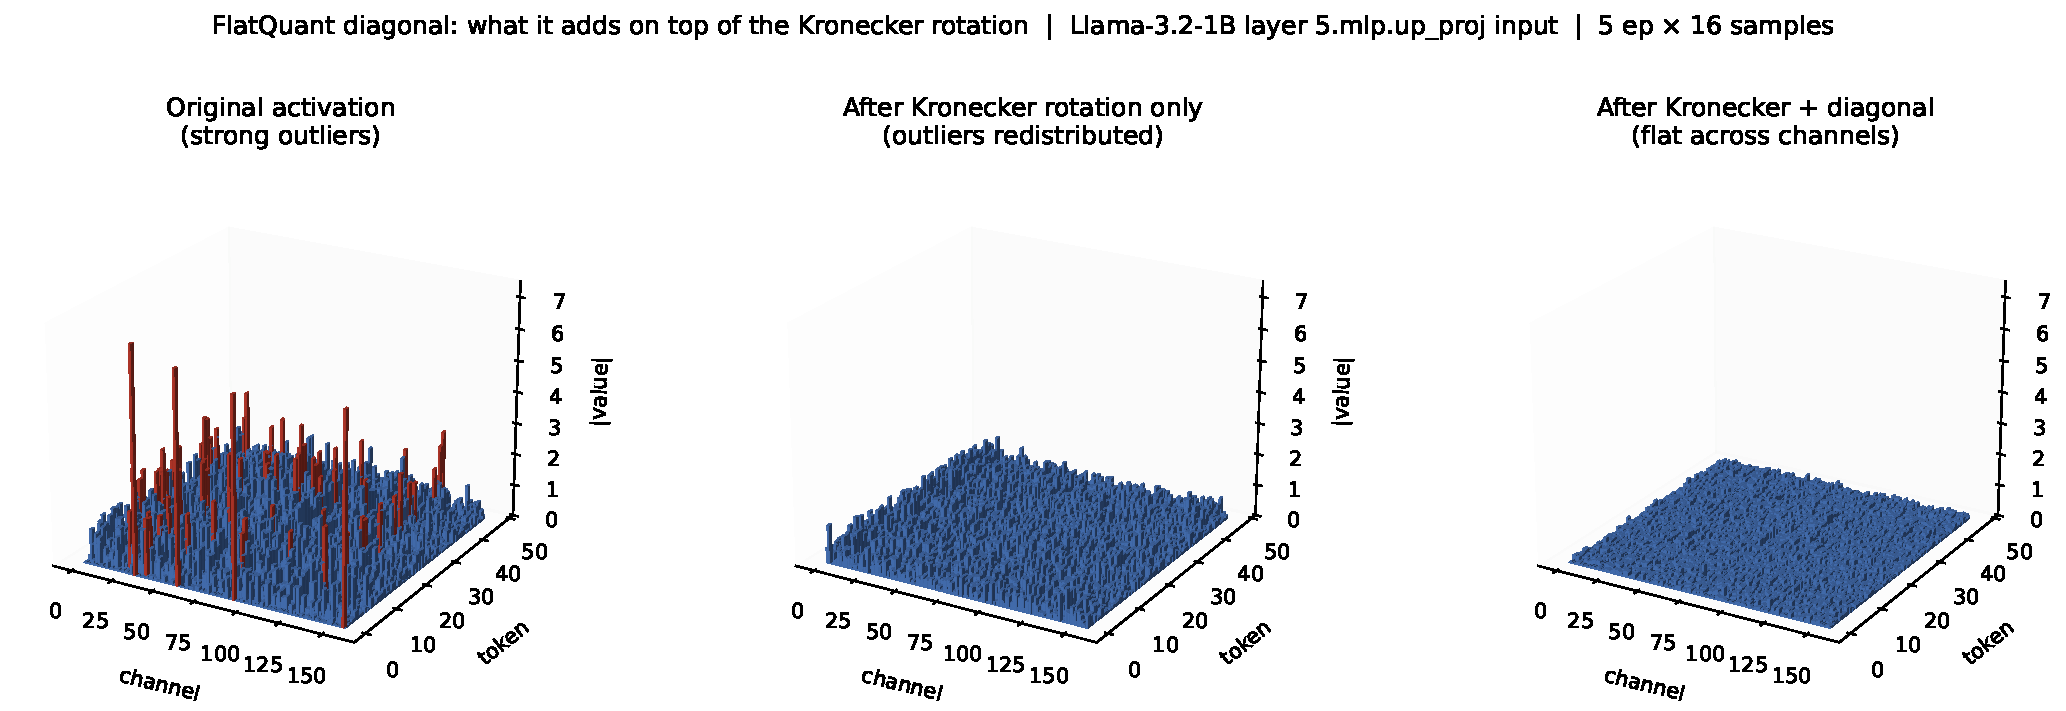
\includegraphics[width=0.95\linewidth]{figs/plot_diag_3d.pdf}
  \end{center}
\end{frame}

% ──────────────────────────────────────────────────────────────────────────────

\begin{frame}{Backup: Staged Training — Why Two Stages?}

  \vfill
  \begin{center}
  \resizebox{0.95\linewidth}{!}{%
  \begin{tikzpicture}[
      every node/.style={font=\footnotesize},
      goalbox/.style={draw=mygray!60, line width=0.7pt, rounded corners=4pt,
                      fill=mygray!8, minimum width=5.4cm, minimum height=1.6cm,
                      align=left, inner sep=8pt},
      arr/.style={-{Latex[length=3mm]}, line width=1.0pt, mygray!70},
    ]

    % ── Two competing observations from ablations ──
    \node[goalbox] (g1) at (-3.2, 1.6) {%
      \textbf{\textcolor{mybluedark}{MLP wants it clean}}\\[0.2em]
      {\scriptsize best \bypass{} with \texttt{diag\_mlp}, $\alpha{=}0$ ---}\\
      {\scriptsize \alert{ADC suffers}.}%
    };

    \node[goalbox] (g2) at (3.2, 1.6) {%
      \textbf{\textcolor{myorange}{Attention wants ADC noise}}\\[0.2em]
      {\scriptsize best \adcppl{} with \texttt{diag\_attn}, $\alpha{\approx}0.5$ ---}\\
      {\scriptsize \alert{no-ADC PPL suffers}.}%
    };

    % ── Conclusion (no box) ──
    \node[align=center, font=\footnotesize] (c) at (0, -1.5) {%
      \textbf{Train sequentially}\;---\;MLP first, then add attention.%
    };

    \draw[arr] (g1.south) -- (c.north -| g1.south);
    \draw[arr] (g2.south) -- (c.north -| g2.south);

  \end{tikzpicture}}
  \end{center}
  \vfill
\end{frame}

% ──────────────────────────────────────────────────────────────────────────────

\begin{frame}[shrink=20]{Backup: Hardware Config \& Delta Formula}
  \begin{columns}[T]
    \begin{column}{0.45\textwidth}
      \begin{center}
      \small
      \begin{tabular}{ll}
        \toprule
        Parameter & Value \\
        \midrule
        $b_w$ (weight bits)   & 4 / 8 \\
        $b_x$ (act.\ bits)    & 4 / 8 \\
        $b_a$ (ADC bits)      & 8 \\
        \texttt{mvm\_limit}   & 256 / 1024 \\
        $k$ (ADC parallelism) & 16 \\
        $\delta$ (mvm=256, INT8) & $\approx 2016$ \\
        $\delta$ (mvm=256, INT4) & $\approx 6.12$ \\
        $\delta$ (mvm=1024, INT8) & $\approx 8064$ \\
        \midrule
        FlatQuant epochs      & 30 \\
        FlatQuant LR          & 0.005 \\
        Cal.\ samples (INT4)  & 1024 \\
        Cal.\ samples (INT8)  & 128 \\
        \bottomrule
      \end{tabular}
      \end{center}
    \end{column}
    \begin{column}{0.50\textwidth}
      \textbf{Delta formula} ($q = 2^{b-1}{-}1$):
      \[
        \delta = \frac{2 \cdot \texttt{tile\_in} \cdot q_x \cdot q_w}{2^{b_a} \cdot k}
      \]
      \begin{itemize}\small
        \item INT8 ($q{=}127$, mvm=256):
              $\frac{2\cdot256\cdot127^2}{256\cdot16}\approx2016$
        \item INT4 ($q{=}7$, mvm=256):
              $\frac{2\cdot256\cdot7^2}{256\cdot16}\approx6.12$
        \item INT8, mvm=1024:
              $\frac{2\cdot1024\cdot127^2}{256\cdot16}\approx8064$
      \end{itemize}

      \vspace{0.1em}
      \textbf{INT8: useful ADC bins} in $\pm\sigma_z \approx 15$--$30$
      (empirical) — explains why INT8 PTQ alone plateaus.
    \end{column}
  \end{columns}
\end{frame}

% ──────────────────────────────────────────────────────────────────────────────

\begin{frame}{Backup: Block-wise Calibration (FlatQuant Baseline)}

  \begin{columns}[T]
    \begin{column}{0.32\textwidth}
      \vspace{1.5em}
      \footnotesize
      \emph{FlatQuant standard.} Train \emph{one block at a time},
      both teacher and student see the \alert{same FP input} $x^\star$:
      \[
        \mathcal L = \bigl\| \hat B(x^\star) - B_{\mathrm{FP}}(x^\star) \bigr\|_2^2
      \]
    \end{column}

    \begin{column}{0.66\textwidth}
      \begin{center}
      \resizebox{!}{0.78\textheight}{%
      \begin{tikzpicture}[
        every node/.style={font=\tiny},
        fbox/.style={draw=mygray!55, dashed, fill=mygray!12, rounded corners=3pt,
                     minimum width=2.5cm, minimum height=0.46cm, align=center},
        tbox/.style={draw=myorange, line width=1.3pt, fill=myorange!22, rounded corners=3pt,
                     minimum width=2.5cm, minimum height=0.46cm, align=center},
        garr/.style={-{Latex[length=1.2mm]}, thick, mygray!65},
        tarr/.style={-{Latex[length=1.2mm]}, thick},
        node distance=0.26cm
      ]
        % ── FP Teacher ────────────────────────────────────────────────
        \node[font=\tiny, text=mygray!80] (l_x)   at (0,    0)   {$x^\star$};
        \node[fbox, above=0.18cm of l_x]  (l_d0)  {Decoder Layer 0};
        \node[fbox, above=of l_d0]        (l_d1)  {Decoder Layer 1};
        \node[fbox, above=of l_d1]        (l_d2)  {Decoder Layer 2};
        \node[font=\small, text=mygray!70, above=0.10cm of l_d2] (l_dots) {$\cdots$};
        \node[fbox, above=0.10cm of l_dots] (l_dN){Decoding Layer N};
        \node[fbox, above=of l_dN]        (l_rms) {RMS Norm.};
        \node[fbox, above=of l_rms]       (l_log) {Logits};
        \node[fbox, above=of l_log]       (l_sm)  {Softmax};
        \node[fbox, above=of l_sm]        (l_prob){Prob.\ dist.};
        \node[font=\tiny\bfseries, text=mybluedark, above=0.18cm of l_prob] {FP Teacher};

        \draw[garr] (l_x)--(l_d0);
        \foreach \a/\b in {l_d0/l_d1, l_d1/l_d2, l_dN/l_rms,
                           l_rms/l_log, l_log/l_sm, l_sm/l_prob}
          \draw[garr] (\a)--(\b);
        \draw[garr] (l_d2)--(l_dots); \draw[garr] (l_dots)--(l_dN);

        \begin{pgfonlayer}{background}
          \node[inner sep=7pt, draw=mygray!40, dashed, fill=mygray!5,
                rounded corners=7pt, fit=(l_x)(l_prob)] {};
        \end{pgfonlayer}

        % ── Quantized Student ─────────────────────────────────────────
        \node[font=\tiny, text=mybluedark] (r_x)  at (4.2,  0)   {$\hat x$};
        \node[tbox, above=0.18cm of r_x]  (r_d0)  {Decoder Layer 0};
        \node[fbox, above=of r_d0]        (r_d1)  {Decoder Layer 1};
        \node[fbox, above=of r_d1]        (r_d2)  {Decoder Layer 2};
        \node[font=\small, above=0.10cm of r_d2] (r_dots) {$\cdots$};
        \node[fbox, above=0.10cm of r_dots] (r_dN){Decoding Layer N};
        \node[fbox, above=of r_dN]        (r_rms) {RMS Norm.};
        \node[fbox, above=of r_rms]       (r_log) {Logits};
        \node[fbox, above=of r_log]       (r_sm)  {Softmax};
        \node[fbox, above=of r_sm]        (r_prob){Prob.\ dist.};
        \node[font=\tiny\bfseries, text=mybluedark, above=0.18cm of r_prob] {Student};

        \draw[tarr] (r_x)--(r_d0);
        \foreach \a/\b in {r_d0/r_d1, r_d1/r_d2, r_dN/r_rms,
                           r_rms/r_log, r_log/r_sm, r_sm/r_prob}
          \draw[garr] (\a)--(\b);
        \draw[garr] (r_d2)--(r_dots); \draw[garr] (r_dots)--(r_dN);

        \begin{pgfonlayer}{background}
          \node[inner sep=7pt, draw=mygray!40, dashed, fill=mygray!5,
                rounded corners=7pt, fit=(r_x)(r_prob)] {};
          \node[inner sep=5pt, draw=myorange!60, fill=myorange!8, rounded corners=5pt,
                fit=(r_d0)] (rb0) {};
        \end{pgfonlayer}

        \draw[decorate, decoration={brace, amplitude=3pt}, myorange]
          (rb0.north east) -- (rb0.south east)
          node[midway, right=4pt, font=\tiny, text=myorange] {trainable};
        \draw[decorate, decoration={brace, amplitude=3pt}, mygray!65]
          (r_prob.north east) -- (r_d1.south east)
          node[midway, right=4pt, font=\tiny, text=mygray] {frozen};

        \draw[{Latex[length=1.2mm]}-{Latex[length=1.2mm]}, thick, myred!75]
          (l_d0.east) -- node[above, font=\tiny, fill=white, inner sep=1pt]
          {$\mathcal{L}$} (r_d0.west);
      \end{tikzpicture}}
      \end{center}
    \end{column}
  \end{columns}
\end{frame}

% ──────────────────────────────────────────────────────────────────────────────
% Copy of slide 6 (07_flatquant.tex) — kept here in backup for Q&A reference.
\begin{frame}{Backup: FlatQuant — Rotate, Flatten, Calibrate per Block}

  \vfill
  \begin{columns}[c]
    \begin{column}{0.46\textwidth}
      \footnotesize
      \textbf{1. Linear invariance.}
      \[
        y \;=\; xW^\top \;=\; \underbrace{(xT^{-1})}_{\tilde x}\underbrace{(TW^\top)}_{\tilde W^\top}.
      \]

      \vspace{0.8em}
      \textbf{2. Kronecker factorisation.}
      \[
        T \;=\; T_1 \otimes T_2,\quad T_1,T_2{\in}\mathbb{R}^{\sqrt d \times \sqrt d}
      \]
    \end{column}

    \begin{column}{0.5\textwidth}
      \footnotesize
      \textbf{3. Teacher-student block-wise calibration.}

      \vspace{0.6em}
      \begin{center}
      \begin{tikzpicture}[every node/.style={font=\tiny}, node distance=0.25cm,
                         box/.style={draw, rounded corners=2pt, minimum width=2.6cm, minimum height=0.45cm, align=center}]
        \node[box, fill=mygray!15] (t) {\textbf{Teacher} layer\\ FP, frozen};
        \node[box, fill=myorange!25, below=0.35cm of t] (s) {\textbf{Student} layer\\ quantised, $T$ trainable};
        \node[right=0.4cm of s, font=\scriptsize] (y2) {$\hat y\phantom{^\star}$};
        \node[font=\scriptsize] (y1) at (y2 |- t) {$y^\star\phantom{\hat{}}$};
        \draw[-{Latex}] (t.east) -- (y1);
        \draw[-{Latex}] (s.east) -- (y2);
        \draw[decorate, decoration={brace, amplitude=3pt}] (y1.east) -- (y2.east) node[midway, right=3pt, font=\scriptsize] {$\|\cdot\|^2$};
      \end{tikzpicture}
      \end{center}
    \end{column}
  \end{columns}
  \vfill
\end{frame}
